\\
In K-means algorithm, the performance of the algorithm is mainly determined by the parameter K, which denotes the number of cluster. However, in most of the situation, it is not possible to determine a proper K. For object recognition, it could be a challenge for human to determine K for the algorithm, even though, human can distinguish objects by some features, such as color, shape, texture, etc. Many works have been done to heuristically determine the number of cluster automatically. Ray et.al \cite{ray1999determination} proposed a method that starts K from 2 to $K_{max}$, which is defined prior as the upper limit for K. Figueiredo et.al. \cite{figueiredo2002unsupervised} estimated K with minimum message length (MML) criteria and Gaussian mixture model. These methods try to learn the data distribution naturally without much human involvement, so it makes the algorithms complicate and slow. 
  \begin{figure}[ht]
    \subfloat[Original Image]{%
      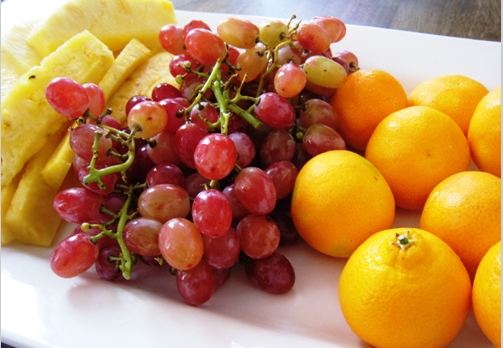
\includegraphics[width=0.45\textwidth]{fig/multdim/orig.png}
    }
    \hfill
    \subfloat[K=5]{%
       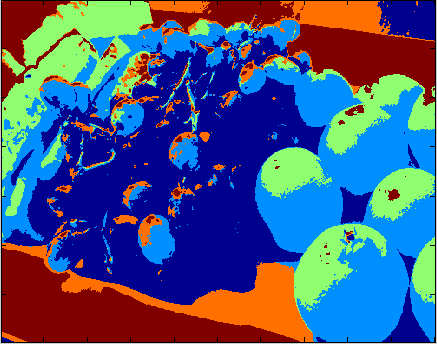
\includegraphics[width=0.45\textwidth]{fig/multdim/k5.png}
    }\\
    \subfloat[K=6]{%
      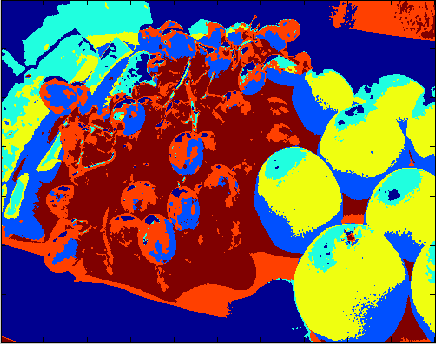
\includegraphics[width=0.45\textwidth]{fig/multdim/k6.png}
    }
    \hfill
    \subfloat[K=10]{%
       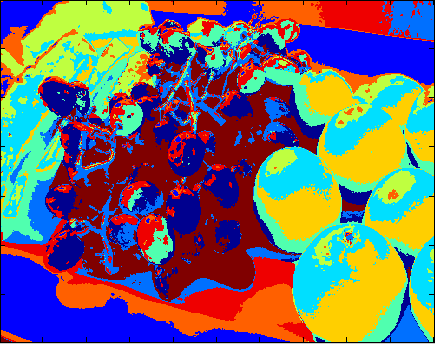
\includegraphics[width=0.45\textwidth]{fig/multdim/k10.png}
    }
    \caption{Clustering for image segmentation}
    \label{fig:cluster seg}
  \end{figure}
  
Normally smaller data can be better clustered while large volume data or data with high dimension could be a hard task for any clustering algorithm. In object recognition, our human classify objects mainly by their shapes and colors. Human have many prior knowledge that can teach the algorithm to use and this could make it simple and fast. Suppose we have to group the two-dimensional dataset in \figref{fig:multidim}.

\begin{figure}[ht]
  \centering
  % Requires \usepackage{graphicx}
  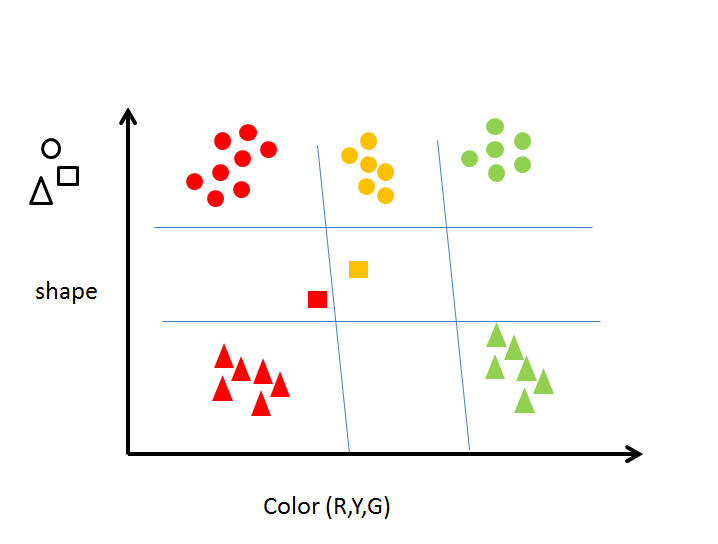
\includegraphics[width=0.7\textwidth]{fig/multdim/example.png}\\
  \caption{How multi-dimensional clustering works}
  \label{fig:multidim}
\end{figure}
